\chapter{Outlook}
\label{chapter:applications}

The presented method for self-collision avoidance is a passive task, which has only constraining purpose. It is not actively actuating any joints to achieve its goal. It is placed on top of the stack in order to monitor the movement of joints and prevent any collisions. 

However, the real impact of the SoT comes visible, when the stack is filled with inequality and equality constraints, and the robot is controlled with the whole body. Thus, in the following chapter, we briefly introduce applications, which we execute on REEM-H. With this, we want to demonstrate the capabilities of the SoT as well as provide an outlook of what is possible with current state of the art humanoid robots.

\subsection*{Object Tracking}
REEM-H possesses a stereo vision system as well as provides support with a Microsoft Kinect RDG-B sensor. With these vision systems we can easily implement an object tracking task. For this, we instantiate an entity, which captures the images from the vision system and provides the position of the object as an output signal. \\
Similarly, we instantiate a gaze task. A gaze task comprises a 2-dimensional plane $\vec{A}$, with a minimal distance $\vec{d}$ to this plane. The task is to keep the orientation of the attached joint $\vec{O}_i$ towards a point $\vec{p}$ on $\vec{A}$. 

Our implementation utilizes already existing components, which are successfully implemented on REEM-H. Related work regarding object recognition was done in \cite{bence}. We performed an object recognition with the help of Aruco markers (see figure \ref{fig:objectrecognition}), which allows an easy positioning of objects, where this marker is attached to.

\begin{figure}[h!]
  \centering
  \subfigure[Gaze Task Illustration]{
  		\label{fig:taskgaze} 
  		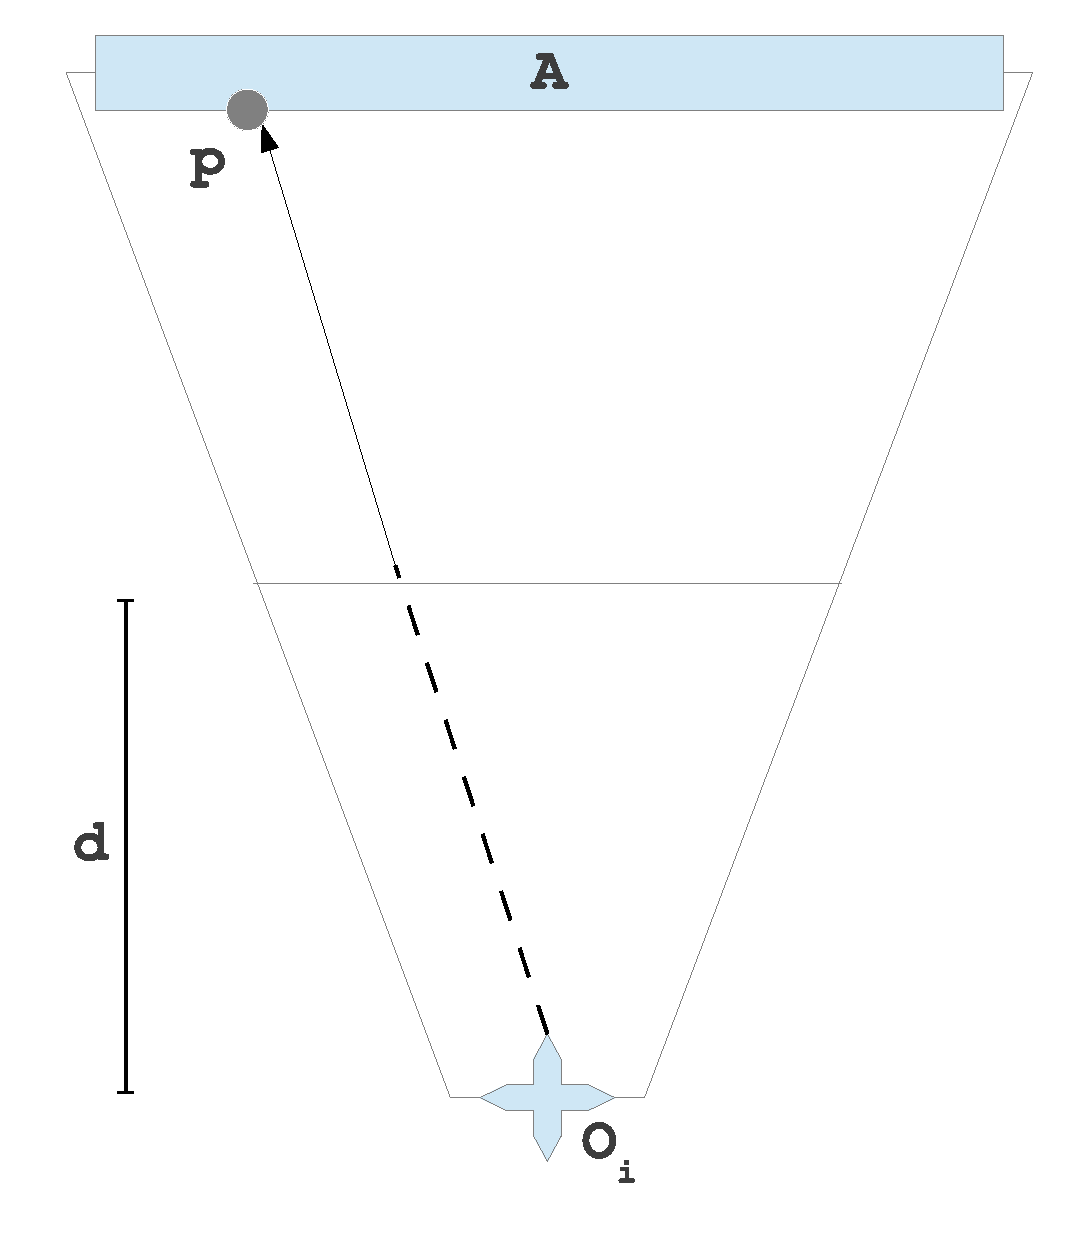
\includegraphics[width=0.4\textwidth]{../figures/gazetask.eps}
  	}
  	\hspace{2cm}
  \subfigure[Aruco Marker]{
  		\label{fig:arucomarker} 
  		\includegraphics[width=0.4\textwidth]{../figures/arucomarker.png}
  	}
	\caption{a) Illustration of a gaze task. The 2-dimensional plane $\vec{A}$, minimal distance $\vec{d}$ and a desired point $\vec{p}$. b) Example Arcuo marker, which is used to extract a full pose or position for various objects.}
    \label{fig:objectrecognition}
\end{figure}

A gaze task can be instantiated as a generic inverse kinematic task, which explicitly requires a Jacobian and a desired goal position for calculating the according error function. Since the vision system is attached at the head link, we plug the Jacobian of the head into the gaze task. The desired value \verb|P| corresponds to the position extraction of the Aruco marker.

\subsection*{Object Grasping}
We previously developed a task for tracking an object through a vision system. The only actuated joints hereby were the ones along the kinematic chain until the head. In order to achieve object grasping, we basically instantiate a positioning task for the end-effector of one arm. Similarly, to the gaze task, we plug the position of the Aruco marker as the desired goal position for this end-effector task. 

However, as in each grasping task, the main difficulty is the way the end-effector approaches the object. If we simply plug the marker position as the desired goal, we might hit the object with the manipulator, while reaching the position. We can overcome this issue by instantiating another gaze task. Contrary to the gaze task of the vision system, the place the gaze in the hand and have it orientate towards the marker. This forces the manipulator to approach the object with a correct grasping orientation.
\newpage
This setup of tasks can be already seen as whole body motion control, since multiple tasks partially share the same joints. Whenever this is the case, hierarchy race conditions occur. It might be dependent on the application, which task has more priority. In our implementation, we foster the head gaze to take precedence over the grasping task, since we want to ensure to have the object in the field of view.

\subsection*{Motion Retargeting}
As second application, we realized motion retargeting inside the SoT. Again, we could reuse existing solutions developed inside PAL \cite{marcus}. Motion retargeting is mainly used to realize teleoperations. Hereby, any RGB-D sensor, such as the Microsoft Kinect, captures a 3-dimensional image of a human and extracts the skeleton image. The idea of motion retargeting is then to translate the extracted joint positions of the human into joint positions of the according robot. Figure \ref{fig:teleop} illustrates the process.

\begin{figure}[h!]
  \centering
  \subfigure[Human movement]{
  		\label{fig:taskgaze} 
  		\includegraphics[width=0.37\textwidth]{../figures/teleop_real.png}
  	}
  \subfigure[Extracted skeleton]{
  		\label{fig:arucomarker} 
  		\includegraphics[width=0.20\textwidth]{../figures/kinect_skeleton.png}
  	}
  	  \subfigure[Translated movement on the robot]{
  		\label{fig:arucomarker} 
  		\includegraphics[width=0.37\textwidth]{../figures/teleop_reem.png}
  	}
	\caption{a) Image of the human movement b) Sketch of the extracted skeleton image c) Translated movement of the human into the robot.}
    \label{fig:teleop}
\end{figure}

We can flexibly realize teleoperations inside the SoT. The skeleton algorithms provides us with cartesian positions for each joint of the robot. Depending on how accurate we want the robot to imitate the movement of the human, we initiate a positioning task for each joint to track. Most often however, it is sufficient to track only the wrist and elbow positions, as the resulting movement of the remaining joints will be resolved quite similarly. 
\newpage
\subsection*{Dynamics}
Throughout this work, we completely worked inside a kinematic domain. This means, we resolved every task with a simple kinematic model in the form of 
\begin{equation}\label{eqn:kinematicmodel}
\vec{\dot{x}} = \vec{J}\vec{\dot{q}}
\end{equation}
This model can be shifted to a dynamics domain, which also considers velocities, inertia and masses to solve joint velocities. \cite{oscar} provides a complete solution to implement dynamics task inside the SoT. The equation in \ref{eqn:kinematicmodel} therefore becomes the Newton-Euler-Equation \cite{dynamics}:
\begin{equation}
\vec{M}(\vec{q}) \vec{\ddot{q}} + \vec{V}(\vec{\dot{q},q}) + \vec{g}(\vec{q}) = \tau
\end{equation}